\chapter{Models of Computation}
\label{cha:models}


A \emph{model of computation} describes what computation is and how it
is done. The best known is Alan Turing's model~\cite{Turing} in which
a machine manipulates the contents of a tape according to a finite set
of instructions. It has become the yardstick with which we measure
other models of computation. Turing's notion of computability is very
robust. First it is robust because changes to the definition of Turing
machines, such as increasing the number of tapes or heads, or allowing
the head to jump around, does not change the computational
power.\footnote{We are ignoring questions of computational
  \emph{complexity}.} The notion is also robust because many other
definitions of computation turned out to be equivalent to Turing's in
the sense that machines of one kind can simulate those of the other
kind, and vice versa.

However, we would commit a serious mistake if we concluded that by
studying only Turing machines we will learn everything there is to
learn about computable mathematics. Our inquiry into the nature of
computation, especially computation with infinite structures, will
reveal a plethora of possibilities which are \emph{not} equivalent.
Thus we begin the chapter with a review of several models of
computation. We then discuss the question of what a model of
computation might be in general, and how such models are compared.


\section{Turing machines}
\label{sec:turing-machines}

We recall informally how a Turing machine operates. There is little
point in giving a formal definition because we do not intend to
actually write programs for Turing machines. If you are not familiar
with Turing machines, see the section on further reading at the end of
the chapter.

\begin{figure}[htbp]
  \centering
  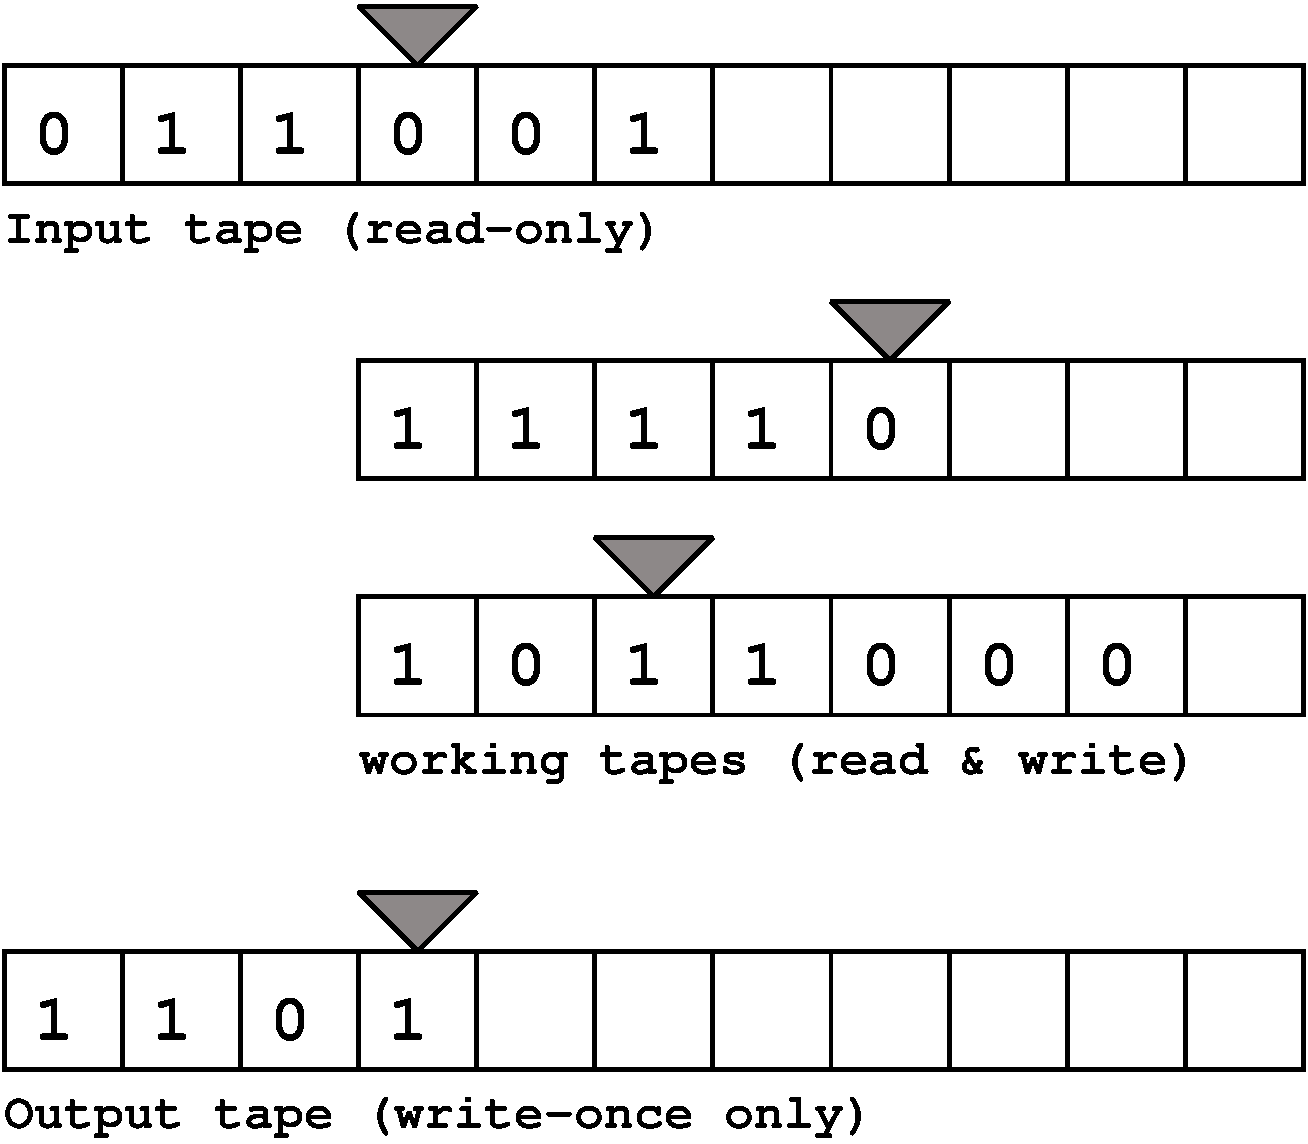
\includegraphics[width=0.5\textwidth]{turing_machine}
  \caption{A Turing machine operates with tapes}
  \label{fig:turing-machine}
\end{figure}

A Turing machine is a device which operates on a number of tapes and
heads, see Figure~\ref{fig:turing-machine}:
%
\begin{itemize}
\item the input tape is equipped with a reading head that can move
  left and right, and read the symbols, but cannot write them.
\item The working tapes are equipped with heads that move left and
  right, and can both read and write symbols.
\item The output tape is equipped with a write-once head which can
  move left and right, and it can write into each cell exactly once.
  Once a cell is filled with a non-blank symbol all subsequent writes
  to it are ignored.
\end{itemize}
%
The tapes are infinite\footnote{If you are worried about having actual
  infinite tapes in your room, note that at each step of the
  computation only a finite portion of tapes has been inspected. In
  this sense the tapes are \emph{potentially} infinite.} and contain
symbols from a given finite alphabet. A common choice for the alphabet
is $0$, $1$, and a special symbol `blank'. The machine manipulates the
contents of the tapes according to a \emph{program}, which is a finite
list of simple instructions that manipulate the heads and the tapes.
The machine executes one instruction at a time in a sequential manner.
It may \emph{terminate} after having executed finitely many
computation steps. If it does not terminate then it runs forever, in
which case we say that it \emph{diverges}.

Our version of Turing machine is different from the usual one, where a
machine is equipped with only a single tape that serves for input,
output, and intermediate work. The two formulations are equivalent in
the sense that a single-tape machine can simulate the workings of a
Turing maechine with several tapes, and vice versa. Our formulation
will ease the description of infinite computations in
Section~\ref{sec:type-2}.

The state of a Turing machine may be encoded onto a single tape as
follows. First we write down the program, suitably encoded by the
symbols from the alphabet, then the current state (the next
instruction to be executed), and positions of the heads. Finally, we
copy the contents of all the tapes by interleaving them into a single
tape.

If we were going to build just one machine, which one would we build?
The answer was given by Turing.

\begin{theorem}[Turing]
  \label{thm:universal-machine}
  There exists a \emph{universal} machine---a machine that takes a
  description of another machine, as explained above, and simulates
  it.
\end{theorem}

\begin{proof}
  A traditional proof may be found in any book on computability
  theory, and there is nothing wrong with reading the original
  proof~\cite{Turing} either. A different kind of a proof is the
  observation that you use universal machines every day.\footnote{You
    have to ignore the fact the several hundred gigabytes of storage
    are not quite the same thing as an infinite tape. Also, modern
    compuers are really universal \emph{Von Neumann}
    machines~\cite{vonNeumann} because they have a central processing
    unit and random access memory instead of a tape.}
\end{proof}

Once we have a universal machine, we can make it behave like any other
machine. It is just
\href{http://www.catb.org/jargon/html/S/SMOP.html}{``a simple matter
  of programming''} to tell it what to do.

We mentioned in the introduction that many kinds of computing devices
are equivalent to Turing machines. We shall therefore not insist on
describing computation solely in terms of Turing machines, but rather
rely on familiarity with modern computers and programming languages.
After all, programs can actually be run on computers, whereas Turing
machines are rather hard to get by.


\subsection{Type 1 machines}
\label{sec:type-1}

How do we use Turing machines to compute a partial\footnote{We use
  notation $f : A \parto B$ to denote a function $f$ which is defined
  on a subset of~$A$ and maps into $B$.} function $f : \NN \parto
\NN$? A natural idea is to write the argument $n$ onto the input tape,
run the machine until it terminates, and read the result $f(n)$ off
the output tape. If the machine diverges then $f(n)$ is undefined. Of
course, the input $n$ must be suitably encoded onto the input tape,
for example it can be written in binary form. Similarly, we expect the
output tape to contain the result encoded in the same manner.

It is convenient to view every Turing machine as one computing a
function $\NN \parto \NN$. This can be arranged as long as we read the
result off the output tape correctly. Suppose the alphabet contains
symbols $0$, $1$ and `blank'. We encode the input $n$ onto the input
tape in binary followed by blanks, and run the machine. If and when it
terminates it has written at most finally many symbols onto the output
tape. Some of the symbols it has written might be different from $0$
and $1$. If we ignore everything that comes after the first blank, we
can interpret the output tape as a number written in binary (the empty
sequence encodes zero).

We could similarly define how a Turing machine computes a multivariate
partial function $f : \NN^k \parto \NN$. We just have to take care
that the input is encoded correctly by placing special markers between
the arguments so that we can tell where one ends and the next one
begins.

It is common knowledge that computers encode everything with $0$'s and
$1$'s, but logicians prefer to encode everything with natural numbers.
For example, a pair of numbers $(m, n)$ may be encoded into a single
number, say $\pair{m, n} = 2^m (2 n + 1)$, in such a way that the
original numbers can be recovered uniquely. We call a computable
function which does this a \emph{pairing function}. The
\emph{projections} $\xfst$ and $\xsnd$ recover $m$ and $n$ from
$\pair{m, n}$, respectively. They are computable as well.

We may also encode Turing machines with numbers. A program is a finite
list of instructions, so it can be encoded as a finite sequence of
$0$'s and $1$'s (your computer does this everytime you save a piece of
source code in a file), which in turn represents a number in binary
form. In fact, every number may be thought of as a code of a program
by the reverse process. Given a number, write it in binary form and
interpret it as a sequence of $0$'s and $1$'s and decode from it a
list of instructions. It may happen that the binary sequence does not
properly encode a list of instructions, in which case we interpret it
as the program that keeps moving the input head to the right forever.

The next step is to encode tapes and entire computations with numbers.
Because an infinite tape cannot be encoded in a single natural number,
we limit attention to the so-called \emph{type 1} machines which
accept only \emph{finite} inputs. More precisely, the input always
consists of a finite string of $0$'s and $1$'s followed by blanks.
Such input may be encoded by a single number. Furthermore, at every
step of computation the machine has used up only a finite portion of
its working tapes. The contents of each tape may be encoded by a
single number, and a finite sequence of numbers $n_0, \ldots, n_k$ may
again be encoded by a single number $[n_0, \ldots, n_k]$, which we can
define as iterated pairing:
%
\begin{align*}
  [] &= 0 \\
  [n_0, \ldots, n_k] &= \pair{n_0, [n_1, \ldots, n_k]}.
\end{align*}
%
Because we defined $\pair{m,n}$ so that it is never zero, the elements
of a sequence may be uniquely reconstructed from its code. By
continuing in this manner we may encode with a single number a finite
sequence of computatation steps, including the contents of the tapes
and positions of the heads at each step. Stephen Kleene~\cite{kleeneT}
worked out the details of all this and defined the predicate
$T(x,y,z)$ whose meaning is
%
\begin{quote}
  ``Machine encoded by $x$ with input tape that encodes the number $y$
  performs a sequence of computation steps encoded by $z$ and
  terminates.''
\end{quote}
%
The amazing thing is that $T$ may be defined in Peano arithmetic just
in terms of basic arithmetical operations on numbers. There is an
associated computable partial function $U(z)$ whose meaning is ``the
number encoded by the contents of the output tape in the last step of
computation encoded by $z$''. The function $U$ allows us to extract
the result of a computation. If $z$ does not encode a terminating
computation then $U(z)$ is undefined.

Kleene's normal form theorem says that every parital computable
function $f : \NN \parto \NN$ may be written in the form
%
\begin{equation}
  \label{eq:kleene-normal-form}
  y \mapsto U(\min \set{z \in \NN \such T(x,y,z)}).
\end{equation}
%
The number $x$ is not uniquely determined, as we may take it to be the
encoding of any machine that computes~$f$. We are completely ignoring
questions of computational efficiency. Just consider how we would
computing $f(y)$ according to~\eqref{eq:kleene-normal-form}: for each
$z = 0, 1, 2, \ldots$, test whether~$z$ encodes a computation of
machine $x$ with input $y$. When you find the first such~$z$, extract
the result $U(z)$ from it. I dare you to compute the constant function
$y \mapsto 0$ this way!

Kleene's normal form may be used to define a standard enumeration of
partial recursive functions. Let
%
\begin{equation*}
  \pr{x}{y} = U(\min \set{z \in \NN \such T(x,y,z)}).
\end{equation*}
%
The sequence $\xpr_0, \xpr_1, \xpr_2, \ldots$ is an enumeration of all
computable partial functions (with repetitions).

The preceding discussion may be generalized to functions of several
variables. For each $k \in \NN$ there is Kleene's predicate
$T^{(k)}(x,y_1,\ldots,y_k,z)$ and the corresponding $U^{(k)}(z)$ that
extracts results from computations. Similarly, there is a standard
enumeration of $k$-place computable partial functions
%
\begin{equation*}
  \prm{k}{x}{y_1, \ldots, y_k} =
  U^{(k)}(\min \set{z \in \NN \such T^{(k)}(x,y_1, \ldots, y_k,z)}).
\end{equation*}
%
These enumerations are not arbitrary. They have the following
important properties, where $a \simeq b$ is \emph{Kleene's equality}
whose meaning is that if one of $a$, $b$ is defined then so is the
other and they are equal.

\begin{theorem}[utm]
  There exists a partial computable function $u : \NN \times
  \NN \parto \NN$ such that, for all $x, y \in \NN$,
  %
  \begin{equation*}
    u(x,y) \simeq \pr{x}{y}.
  \end{equation*}
\end{theorem}

\begin{theorem}[smn]
  For each $n$ and $m$ there exists a computable function $s_n^m :
  \NN^{m+1} \to \NN$ such that, for all $x, y_1, \ldots, y_m, z_1,
  \ldots, z_n \in \NN$,
  %
  \begin{equation*}
    \prm{n}{s_n^m(x,y_1, \ldots, y_m)}{z_1, \ldots z_n} \simeq
    \prm{n+m}{x}{y_1, \ldots, y_m, z_1, \ldots, z_m}.
  \end{equation*}
\end{theorem}

\noindent
The utm theorem is essentially a restatement of
Theorem~\ref{thm:universal-machine} in terms of computable partial
functions. A detailed proof of the utm and smn theorems would involve
a lot of technical manipulations of Turing machines. Rather than
losing time with such a historical exercise, let us see how these two
theorems manifest themselves in modern programming languages, say in
Haskell. Keeping in mind that numbers are just codes for programs and
data, the universal function $u$ from the utm theorem is
%
\begin{lstlisting}[language=Haskell]
u (f, y) = f y
\end{lstlisting}
%
and the $s_n^m$ function for the case $n = m = 1$ is the currying
operation\footnote{In Haskell the notation \texttt{{\char92}x -> e}
  stands for $\lambda$-abstraction $\xulam{x}{e}$, which in turn means
  ``the function which maps $x$ to $e$''.}
%
\begin{lstlisting}[language=Haskell]
s (f, y) = \z -> f (y, z)
\end{lstlisting}
%
This may seem like a triviality to the programmer but is surely not
considered one by those who implemented the Haskell compiler.
Application and currying are ``the essence'' of functional
programming, just like the utm and smn theorems are the essence of
partial computable functions.

We finish this section with a theorem which we shall often use to show
\emph{non}-computability results.

\begin{theorem}[Halting oracle]
  The \emph{halting oracle},
  %
  \begin{equation*}
    h(x) =
    \begin{cases}
      1 & \text{if $\pr{x}{0}$ is defined,}\\
      0 & \text{if $\pr{x}{0}$ is not defined,}
    \end{cases}
  \end{equation*}
  %
  is \emph{not} computable.
\end{theorem}

\begin{proof}
  Let us prove the theorem in Haskell. We must show that there is no
  %
  \begin{lstlisting}[language=Haskell]
h :: (Integer -> Integer) -> Integer
  \end{lstlisting}
  %
  such that, for all \lstinline!f :: Integer -> Integer!,
  %
  \begin{equation*}
    \text{\lstinline!h f!} =
    \begin{cases}
      \text{\lstinline!1!} & \text{if \lstinline!f 0! terminates,}\\
      \text{\lstinline!0!} & \text{if \lstinline!f 0! diverges.}
    \end{cases}
  \end{equation*}
  %
  Suppose there were such an \lstinline!h!. Define
  %
  \begin{lstlisting}[language=Haskell]
g n = if h g == 1 then g n else 0
  \end{lstlisting}
  %
  By assumption \lstinline!h g! is either \lstinline!0! or
  \lstinline!1!. In either case there is a contradiction because
  \lstinline!g! does just the opposite of what \lstinline!h! says it
  will do.
\end{proof}


\subsection{Type 2 machines}
\label{sec:type-2}

Type 1 machines from previous section only operate on finite inputs.
In practice we often see programs whose input and output are
(potentially) infinite. For example, when you listen to an internet
radio station, the player accepts a never-ending stream of data which
it outputs to the speakers. Also, just because a program does not
terminate that does not automatically make it useless. We therefore
also need a model of computation that describes non-terminating
programs with infinite inputs and outputs.

A popular one is \emph{type 2} Turing machine, which accepts an
infinite sequence on its input tape and is allowed to work forever. It
may or may not fill the output tape entirely with non-blank symbols.
Note that the requirement for the output tape to be write-once makes
it possible to tell when the machine has actually produced an output
in a given cell. Had we allowed the machine to write to each output
cell many times, it could keep coming back and changing what it has
already written.

An important distinction between type 1 and type 2 machines is that
the latter may accept non-computable inputs, from which non-computable
outputs may be produced.

For type 2 machines there are analogoues of the standard
enumeration~$\xpr$, utm and the smn theorems. These are more easily
expressed if we allow the machines to write natural numbers in the
cells, rather than symbols from a finite alphabet. We also need equip
the machines with instructions for manipulating the numbers written in
the cells, say, instructions for manipulating the bits and for testing
equality with zero. These changes are inessential because an infinite
sequence $n_0, n_1, n_2, \ldots$ of natural numbers may be encoded as
a binary sequence $1^{n_0}01^{n_1}01^{n_2}0\cdots$, where $1^k$ means
that the symbol $1$ is repeated $k$-times.

A type 2 machine computes a partial function $f : \NN^\NN \parto
\NN^\NN$, where $\NN^\NN$ is the \emph{Baire space} of infinite
sequences of numbers. We run the machines with $\alpha \in \NN^\NN$
written on the input tape. If the machine eventually writes a number
to every output cell, then $f(\alpha)$ is the resulting sequence. If
there is at least one output cell to which the machine does not write
a number, then $f(\alpha)$ is undefined.

We may similarly define what it means for a machine to compute a
multivariate parital function $f : (\NN^\NN)^k \parto \NN^\NN$. The
input $(\alpha_1, \ldots, \alpha_k)$ is written onto the input tape in
an interleaving manner, so that $\alpha_{i,j}$ is found in the cell at
position $k \cdot j + i$.

Before proceeding with type 2 computability, we recall a few basic
facts about the Baire space~$\Baire = \NN^\NN$. Let $\NN^{*}$ be the
set of all finite sequences of natural numbers. If $a, b \in \NN^{*}$
we write $a \sqsubseteq b$ when $a$ is a prefix of~$b$. The length of
a finite sequence $a$ is denoted by~$|a|$. Similarly, we write $a
\sqsubseteq \alpha$ when $a$ is a prefix of an infinite sequence
$\alpha \in \Baire$. A finite prefix $\alpha_0, \ldots, \alpha_{k-1}$
of $\alpha$ may be encoded by a single number $\seg{a}{n} = [\alpha_0,
\ldots, \alpha_{k-1}]$.

The expression $\cons{a}{\beta}$ denotes the concatenation of the
finite sequence $a \in \NN^{*}$ with the infinite sequence $\beta \in
\Baire$. Sometimes we abuse notation and write $\cons{n}{\beta}$
instead of $\cons{\seq{n}}{\beta}$ for $n \in \NN$ and $\beta \in
\Baire$.

We equip $\Baire$ with the product topology. A countable topological
base for $\Baire$ consists of the basic open sets
%
\begin{equation*}
  \cons{\seq{a_0, \ldots, a_k}}{\Baire}
  = \set{\cons{\seq{a_0, \ldots, a_{k-1}}}{\beta} \such \beta \in \Baire}
  = \set{\alpha \in \Baire \such \seq{a_0, \ldots, a_{k-1}}
    \sqsubseteq \alpha}
  \;.
\end{equation*}
%
Because the basic open sets are both closed and open (clopen),
$\Baire$ is in fact a countably based $0$-dimensional\footnote{Recall
  that a space is \emph{$0$-dimensional} when its clopen subsets form
  a base for its topology.} Hausdorff space. It is also a complete
separable metric space for the \emph{comparison metric} $d : \Baire
\times \Baire \to \RR$, defined by
%
\begin{equation*}
  d(\alpha, \beta) = \inf \;\set{2^{-n} \such
    \seg{\alpha}{n} = \seg{\beta}{n}}.
\end{equation*}
%
If the first term in which $\alpha$ and $\beta$ differ is the $n$-th
one, then $d(\alpha, \beta) = 2^{-n}$. The comparison metric is an
ultrametric, which means that it satisfies the inequality $d(\alpha,
\gamma) \leq \max(d(\alpha, \beta), d(\beta, \gamma)$. The clopen sets
$\cons{a}{\Baire}$ are balls of radius $2^{-|a|}$.

Let us now see how encoding of partial computable functions works. We
would like to encode a computable $f : \Baire \parto \Baire$ with an
element $\beta \in \Baire$. Suppose that, given input $\alpha \in
\Baire$, the machine which computes $f$ writes $j$ to the $i$-th
output cell after $k$ steps of computation. This means that
$f(\alpha)_i = j$. Because in~$k$ steps the machine inspects at most
the first $k$ input cells, it would have done the same for any other
input that agrees with $\alpha$ in the first $k$ terms. This gives us
the idea that $\beta$ should carry bits of information of the form
%
\begin{quote}
  ``if the input tape starts with $\alpha_0, \ldots,
  \alpha_{k-1}$ then the machine writes $j$ in the $i$-th input
  cell.''
\end{quote}
%
More precisely, we compute $\beta_m$ as follows. First decode~$m$ as
$\seq{i, n_0, \ldots, n_{k-1}}$. (The number $m = 0$ encodes the empty
sequence and cannot be so decoded, so we set $\beta_0 = 0$.) Then
simulate the machine for $k$ steps with input tape $n_0, \ldots,
n_{k-1}, 0, 0, \ldots$. If the machine writes $j$ into the $i$-th
output cell during the simulation, set $\beta_m = j + 1$, otherwise
set $\beta_m = 0$.

Conversely, every $\beta \in \Baire$ detemines a partial function $f :
\Baire \parto \Baire$, defined by
%
\begin{equation}
  \label{eq:type2-encoding}
  f(\alpha)_i = \beta_m - 1
  \qquad\text{where}\qquad
  m = \min\nolimits_m (\xsome{i,k}{\NN}{m = \seg{(\cons{i}{\alpha})}{k}} \land
    \beta_m \neq 0).
\end{equation}
%
The function which $\beta$ encodes is denoted by $\xfpr_\beta$. A
partial map of of the form $\xfpr_\beta$ is said to be \emph{(type 2)
  realizable}. We would like to know which maps are realizable.

A partial function $f: X \parto Y$ is said to be \emph{continuous}
when it is continuous as a total map $f: \dom{f} \to Y$, where the
domain of definition $\dom{f} \subseteq X$ is equipped with the
subspace topology. Note that there is no restriction on the
domain~$\dom{f}$.

\begin{theorem}[Extension Theorem for $\Baire$]
  \label{th:extension_BB}%
  Every partial continuous map $f: \Baire \parto \Baire$ can be extended
  to a realized one.
\end{theorem}

\begin{proof}
  Suppose $f: \Baire \parto \Baire$ is a partial continuous map.  Consider
  the set $A \subseteq \NN^{*} \times \NN^2$ defined by
  %
  \begin{equation*}
     A = \set{(a, i, j) \in \NN^{*} \times \NN^{2} \such
        \cons{a}{\Baire} \cap \dom{f} \neq \emptyset \land
        \all{\alpha}{\cons{a}{\Baire} \cap \dom{f}}{
          (f\alpha)_i = j
          }
        }
  \end{equation*}
  %
  If $(a, i, j) \in A$, $(a', i, j') \in A$ and $a \sqsubseteq a'$
  then $j = j'$ because there exists $\alpha \in \cons{a'}{\Baire}
  \cap \dom{f} \subseteq \cons{a}{\Baire} \cap \dom{f}$ such that $j =
  (f \alpha)_i = j'$. We define a sequence $\phi \in \Baire$ as
  follows. For every $(a, i, j) \in A$ let $\phi_{\seq{\cons{i}{a}}} =
  j + 1$, and for all other arguments $n$ let $\phi_n = 0$. Suppose
  that $\phi_{\seq{\cons{i}{a}}} = j + 1$ for some $i, j \in \NN$ and
  $a \in \NN^{*}$. Then for every prefix $a' \sqsubseteq a$,
  $\phi_{\seq{\cons{i}{a'}}} = 0$ or $\phi_{\seq{\cons{i}{a'}}} = j +
  1$. Thus, if $(a, i, j) \in A$ and $a \sqsubseteq \alpha$ then
  $(\fpr{\phi}{\alpha})_i = j$.
  %
  We show that $(\fpr{\phi}{\alpha})_i = (f(\alpha))_i$ for all
  $\alpha \in \dom{f}$ and all $i \in \NN$. Because~$f$ is continuous,
  for all $\alpha \in \dom{f}$ and $i \in \NN$ there exists $(a, i, j)
  \in A$ such that $a \sqsubseteq \alpha$ and $(f \alpha)_i = j$. Now
  we get
  %
  $
    (\fpr{\phi}{\alpha})_i
    = j
    = (f \alpha)_i
  $.
\end{proof}

\index{set!G-delta set@{$G_\delta$}}%
%
Recall that a $G_\delta$-set is a countable intersection of open sets.

\begin{proposition}
  \label{th:G_delta_characteristic}%
  If $U \subseteq \Baire$ is a $G_\delta$-set then the partial
  function $u: \Baire \parto \Baire$ whose domain is $U$ and is
  defined by $u(\alpha)_i = 1$, is realized.
\end{proposition}

\begin{proof}
  The set $U$ is a countable intersection of countable unions of basic
  open sets
  %
  \begin{equation*}
    U = \bigcap_{i \in \NN}
        \bigcup_{j \in \NN} \cons{a_{i,j}}{\Baire} \;.
  \end{equation*}
  %
  Define a sequence $\upsilon \in \Baire$ by setting
  $\upsilon_{\seq{\cons{i}{a_{i,j}}}} = 2$ for all $i, j \in \NN$, and
  $\upsilon_n = 0$ for all other arguments~$n$. Clearly, if
  $\fpr{\upsilon}{\alpha}$ is defined then its value is the constant
  sequence $1, 1, 1, \ldots$, so we only need to verify that
  $\dom{\xfpr_\upsilon} = U$. If $\alpha \in \dom{\xfpr_\upsilon}$
  then $\upsilon \star (\cons{i}{\alpha})$ is defined for every $i \in
  \NN$, therefore there exists $c i \in \NN$ such that $\upsilon
  (\seq{(\cons{i}{[\alpha 0, \ldots, \alpha (c i)]})}) = 2$, which
  implies that $\alpha \in {a_{i, c i}}$. Hence
  %
  \begin{equation*}
    \alpha \in \bigcap_{i \in \NN} \cons{a_{i, c i}}{\Baire} \subseteq U.
  \end{equation*}
  %
  Conversely, if $\alpha \in U$ then for every $i \in \NN$ there
  exists some $c i \in \NN$ such that $\alpha \in a_{i, c i}$. For
  every $i \in \NN$, $\upsilon (\seq{(\cons{i}{[\alpha 0, \ldots,
      \alpha (c i)]})}) = 2$, therefore $(\fpr{\upsilon}{\alpha}) i =
  \upsilon \star (\cons{i}{\alpha}) = 1$.  Hence $\alpha \in
  \dom{\xfpr_\upsilon}$.
\end{proof}


\begin{corollary}
  \label{th:restrict_G_delta}%
  Suppose $\alpha \in \Baire$ and $U \subseteq \Baire$ is a $G_\delta$-set.
  Then there exists $\beta \in \Baire$ such that $\xfpr{\alpha}{\gamma} =
  \fpr{\beta}{\gamma}$ for all $\gamma \in \dom{\xfpr_\alpha} \cap U$ and
  $\dom{\xfpr_\beta} = U \cap \dom{\xfpr_\alpha}$.
\end{corollary}

\begin{proof}
  By Proposition~\ref{th:G_delta_characteristic} there exists
  $\upsilon \in \Baire$ such that for all $\beta \in \Baire$
  %
  \begin{equation*}
    \fpr{\upsilon} \beta =
    \begin{cases}
      \xulam{n}{1} & \beta \in U \;,\\
      \text{undefined} & \text{otherwise} \;.
    \end{cases}
  \end{equation*}
  %
  It suffices to show that the function $f: \Baire \parto \Baire$ defined by
  %
  \begin{equation*}
    (f \beta) n = ((\eta_{\upsilon} \beta) n) \cdot
                  ((\eta_{\alpha} \beta) n)
  \end{equation*}
  %
  is realized. This is so because coordinate-wise multiplication of
  sequences is realized, and so are pairing and composition.
\end{proof}


\begin{theorem}
  \index{realized function!characterization in B@{characterization in~$\kltwo$}}%
  %
  A partial function $f: \Baire \parto \Baire$ is realized if, and only
  if, $f$ is continuous and its domain is a $G_\delta$-set.
\end{theorem}

\begin{proof}
  First we show that $\xfpr_\alpha$ is a continuous map whose domain
  is a $G_\delta$-set. It is continuous because the value of
  $(\fpr{\alpha}{\beta}) n$ depends only on $n$ and finite prefixes of
  $\alpha$ and $\beta$. The domain of $\xfpr_\alpha$ is the
  $G_\delta$-set
  %
  \begin{multline*}
    \dom{\fpr{\alpha}}
    = \set{\beta \in \Baire \such
      \all{n}{\NN}{(\alpha \mid \beta) n\ \text{defined}}} \\
    = \bigcap_{n \in \NN}
      \set{\beta \in \Baire \such (\alpha \mid \beta) n \ 
        \text{defined}}
    =  \bigcap_{n \in \NN}
        \bigcup_{m \in \NN}
          \set{\beta \in \Baire \such
          \alpha \star (\cons{n}{\beta}) = m} \;.
  \end{multline*}
  %
  Each of the sets $\set{\beta \in \Baire \such \alpha \star
    (\cons{n}{\beta}) = m}$ is open because $\star$ and $\cons{}{}$
  are continuous operations.
  
  Now let $f: \Baire \parto \Baire$ be a partial continuous function whose
  domain is a $G_\delta$-set. By Theorem~\ref{th:extension_BB} there
  exists $\phi \in \Baire$ such that $f \alpha = \fpr{\phi} \alpha$ for
  all $\alpha \in \dom{f}$. By Corollary~\ref{th:restrict_G_delta}
  there exists $\psi \in \Baire$ such that $\dom{\fpr{\psi}} = \dom{f}$
  and $\fpr{\psi} \alpha = \fpr{\phi} \alpha$ for every $\alpha \in
  \dom{f}$.
\end{proof}

Finally, we formulate the utm and smn theorems for type 2 machines.

\begin{theorem}[type 2 utm]
  There exists a computable partial function $u : \Baire \times
  \Baire \parto \Baire$ such that $u(\alpha, \beta) \simeq
  \fpr{\alpha}{\beta}$ for all $\alpha, \beta \in \Baire$.
\end{theorem}

\begin{proof}
  Let us write a machine for computing $u$ in Haskell, but without
  resorting to an explicit encoding of finite sequences by numbers.
  Define the type
  %
  \begin{lstlisting}
type Baire = Integer -> Integer
  \end{lstlisting}
  %
  The universal \lstinline!u :: ([Integer] -> Integer, Baire) -> Baire! %
  is just the transliteration of~\eqref{eq:type2-encoding}:
  %
  \begin{lstlisting}[language=Haskell]
u (a, b) i = x - 1
    where x = head $
              filter (/= 0) $
              [a (i : map b [0..(k-1)]) | k <- [0..]]
  \end{lstlisting}
  % 
  You may entertain yourself by learning Haskell and figuring out how
  it works.
\end{proof}

We only bother to state the type 2 version of smn theorem for
bivariate functions.

\begin{theorem}[type 2 smn]
  There exists a computable $s : \Baire \times \Baire \to \Baire$ such
  that, for all $\alpha, \beta, \gamma \in \Baire$,
  %
  \begin{equation*}
    \fprm{2}{s(\alpha, \beta)}{\gamma} = \fpr{\alpha}(\beta, \gamma).
  \end{equation*}
\end{theorem}

\begin{proof}
  The proof is left as an exercise in programming.
\end{proof}


%%%%%%%%%%%%%%%%%%%%%%%%%%%%%%%%%%%%%%%%%%%%%%%%%%
\section{The graph model}
\label{sec:graph-model}

A model of computation may introduce features which are not easily
detected, until we compare it with other models. For example, the
innocuous-looking idea that the input be stored on a tape gives a type
2 machine the ability to take into account the \emph{order} in which
data is stored. In this section we consider a different model of
infinite computation, the \emph{graph model} introduced by Dana
Scott~\cite{graph-model}, in which we use sets of numbers rather than
sequences.

We would like to explain what it means to compute a map $f : \pow{\NN}
\to \pow{\NN}$ where $\pow{\NN}$ is the powerset of natural numbers.
One natural idea would be to use computation with respect to an
oracle: $f$ is computable if there is a Turing machine which computes
$f(A)$ when given $A$ as an oracle, i.e., it may test membership
in~$A$. However, this is still just type 2 computability in disguise,
because asking an oracle whether a number belongs to~$A$ is equivalent
to having an infinite input tape with a $1$ in the $n$-th cell when $n
\in A$, and a $0$ otherwise.

An oracle provides both \emph{positive} and \emph{negative}
information about membership in~$A$, whereas the graph model keeps
only positive information. Rather than describing it explicitly as a
kind of Turing machines, we shall take a different route this time and
first describe the topological aspects of the model. Computability
will then follow easily.

The set $\pow{\NN}$ may be equipped with a topology in two natural
ways. One is the product topology arising from the observation that
$\pow{\NN}$ is isomorphic to the countable product $\two^\NN$. This
topology encodes positive and negative information. The other is the
\emph{Scott} topology, which arises from the lattice structure of
$\pow{\NN}$, ordered by $\subseteq$. A subbasic open set for the Scott
topology on $\pow{\NN}$ is one of the form
%
\begin{equation*}
  \upper{n} = \set{A \subseteq \NN \such n \in A}.
\end{equation*}
%
By forming finite intersections we get the basic open sets
%
\begin{equation*}
  \upper{\set{n_0, \ldots, n_{k-1}}} =
  \set{A \subseteq \NN \such \set{n_0, \ldots, n_{k-1}} \subseteq A}.
\end{equation*}
%
A subset $\mathcal{U} \subseteq \pow{\NN}$ is then \emph{Scott open}
when it has the property that $A$ is a member of~$\mathcal{U}$ if, and
only if, some finite subset of $A$ is a member of $\mathcal{U}$. If we
write $A \wayb B$ when~$A$ is a finite subset of~$B$, we may express
the fact that $\mathcal{U} \subseteq \pow{\NN}$ is Scott open as
%
\begin{equation*}
  not finished here.
\end{equation*}
%
The Scott topology makes $\pow{\NN}$ into a countably based
$T_0$-space, i.e., for all $A, B \in \pow{\NN}$,
%
\begin{equation*}
  \text{$A$ and $B$ have the same neighborhoods} \implies A = B.
\end{equation*}
%
This is \emph{not} a Hausdorff space, not even a $T_1$-space. If you
were taught in school by geometrically minded topologists to ridicule
non-Hausdorff spaces\footnote{I surely was as an undergraduate student
  in mathematics.}, you better quickly lose the habit and learn about
the role of topology as an aspect of information processing in which
an open set is a (positively) observable property. The natural
separation axiom in this setting is~$T_0$, which is a form of
Leibniz's principle of identity.\footnote{The principle states that
  two things are equal if they have exactly the same properties.} We
denote $\pow{\NN}$ by $\Scott$ when we think of it as a topological
space equipped with the Scott topology.

\begin{proposition}
  The following are equivalent for a map $f : \Scott \to \Scott$:
  %
  \begin{enumerate}
  \item $f$ is continuous,
  \item $f(B) = \tbigcup \set{f(A) \such A \wayb B}$ for all $B \in \Scott$,
  \item $f$ preserves directed unions.
  \end{enumerate}
\end{proposition}

\begin{proof}
  A map $f : \Scott \to \Scott$ is continuous precisely when the
  inverse image of a subbasic open set $\invim{f}(\upper{n})$ is open.
  By noting that $B \in \invim{f}(\upper{n})$ is equivalent to $n \in
  f(B)$ and using the characterization of Scott open sets, we may
  phrase continuity of $f$ as
  %
  \begin{equation*}
    \xall{n}{\NN}{
      \all{B}{\Scott}{
        n \in f(B) \iff \xusome{A \wayb B}{n \in f(A)}
      }
    }.
  \end{equation*}
  %
  This is equivalent to saying that, for all $B \in \Scott$,
  %
  \begin{equation*}
    f(B) = \tbigcup \set{f(A) \such A \wayb B}.
  \end{equation*}
  %
  We have proved the equivalence of the first two statements. Since
  $\set{A \such A \wayb B}$ is a directed family, the third statement
  obviously implies the first one. The remaining implication is
  established as follows. Suppose $f : \Scott \to \Scott$ satisfies
  the second statement and $\mathcal{F} \subseteq \Scott$ is a
  directed family. Observe that the families $\mathcal{G} = \set{A \in
    \Scott \such \xsome{B}{\mathcal{F}}{A \wayb B}}$ and $\mathcal{H}
  = \set{A \in \Scott \such A \wayb \tbigcup \mathcal{F}}$ are
  actually the same, both are directed, and $\tbigcup \mathcal{F} =
  \tbigcup \mathcal{H}$. Then
  %
  \begin{align*}
    f (\tbigcup \mathcal{F}) &=
    \tbigcup \set{f(A) \such A \wayb \tbigcup \mathcal{F}} \\
    &= \tbigcup \set{f(A) \such A \in \mathcal{H}} \\
    &= \tbigcup \set{f(A) \such A \in \mathcal{G}} \\
    &= \tbigcup \set{\tbigcup \set{f(A) \such A \wayb B} \such B \in \mathcal{F}} \\
    &= \tbigcup \set{f(B) \such B \in \mathcal{F}}.
  \end{align*}
  %
  We used the second statement in the first and last line.
\end{proof}

A continuous map on $\Scott$ is also called an \emph{enumeration
  operator}. The second part of the previous proposition tells us that
every enumeration operator is determined by its values on finite sets.
This gives us the idea that it should be possible to encode it by a
set of numbers. Indeed, to every continuous $f : \Scott \to \Scott$ we
assign its \emph{graph}
%
\begin{equation*}
  \Gamma(f) = \set{\pair{[m_0, \ldots, m_{k-1}], n} \in \NN \such
    n \in f(\set{m_0, \ldots, m_{k-1}})
  }.
\end{equation*}
%
To every $A \in \Scott$ we assign a function $\Lambda(A) : \Scott \to
\Scott$, defined by
%
\begin{equation*}
  \Lambda(A)(B) = \set{n \in \NN \such
    \xsome{m_0, \ldots, m_{k-1}}{B}{\pair{[m_0, \ldots, m_{k-1}], n} \in A}
  }.
\end{equation*}
%
It is easy to verify that $\Lambda(A)$ is continuous and that
%
\begin{equation*}
  \xymatrix{
    **[l]{\mathcal{C}(\Scott, \Scott)}
    \ar@<+0.25em>[r]^{\Gamma}
    &
    {\Scott}
    \ar@<+0.25em>[l]^{\Lambda}
  }
\end{equation*}
%
is a continuous section-retraction pair which embeds the space of
continuous maps $\mathcal{C}(\Scott, \Scott)$ into $\Scott$. Here
$\mathcal{C}(\Scott, \Scott)$ is equipped with the compact-open
topology.

Let us now discuss the role of $\Scott$ as a model of computation. A
\emph{computably enumerable (c.e.) set} $A \subseteq \NN$ is a one
that can be enumerated by a Turing machine, i.e., it is the image of a
partial computable function $\NN \parto \NN$.\footnote{We must allow
  partial functions if we want the empty set to be computably
  enumerable.} We denote the family of c.e.~sets by $\cScott$. We say
that an enumeration operator $f : \Scott \to \Scott$ is
\emph{computable} if its graph $\Gamma(f)$ is a c.e.~set.

There is a pairing function $\pair{{-}, {-}} : \Scott \times \Scott
\to \Scott$ which interleaves sets $A$ and $B$ as odd and even
numbers, respectively,
%
\begin{equation*}
  \pair{A, B} = \set{2 m \such m \in A} \cup \set{2 n + 1 \such n \in B}.
\end{equation*}
%
This is actually a homeomorphism between $\Scott \times \Scott$ and
$\Scott$. We are not going to bother formulating the utm and smn
theorems for the graph model because we will see later that they hold
in a much more general context.

%%%%%%%%%%%%%%%%%%%%%%%%%%%%%%%%%%%%%%%%%%%%%%%%%%
\section{$\lambda$-calculus and its models}
\label{sec:lambda-calculus}

The $\lambda$-calculus is a theory of functions. The two basic
operations of the calculus are \emph{application} of a function to an
argument and function formation by \emph{abstraction}.

\subsection{Untyped $\lambda$-calculus}
\label{sec:untyped-lambda-calculus}

In the \emph{untyped} version no restrictions are imposed on these
operations. More precisely, the calculus consists of:
%
\begin{itemize}
\item An infinite supply of variables $x, y, z, \ldots$,
\item For any expressions $e_1$ and $e_2$ we may form their
  application $e_1\, e_2$. Application associates to the left so that
  $e_1\, e_2\, e_3 = (e_1\, e_2)\, e_3$.
\item If $e$ is an expression, then $\xulam{x}{e}$ is its abstraction,
  where~$x$ is bound in~$e$. Think of $\xulam{x}{e}$ as the function
  which maps $x$ to $e$. We abbreviate a nested abstraction
  $\xulam{x_1}{\cdots \xulam{x_n}{e}}$ as $\xulam{x_1 x_2 \ldots x_n}{e}$.
\end{itemize}
%
We consider expressions which only differ in the naming of bound
variables as equal. Thus $\xulam{x}{y\, x} = \xulam{z}{y\, z} \neq
\xulam{y}{y\, y}$.

Substitution is an operation which replaces free variables with
expresions. We write $\subst{e}{x_1 \mapsto e_1, \ldots, x_n \mapsto
  e_n}$ for a simultaneous subtitution of expressions $e_1, \ldots,
e_n$ for varaibles $x_1, \ldots, x_n$ in $e$, respectively. The usual
rules for bound variables must be observed when we perform
subtitutions.\footnote{It is notoriously easy to commit errors when
  defining the details of substitution. The best way to understand all
  the intricacies is to write a program that performs substitutions.}

The basic axiom of $\lambda$-calculus is \emph{$\beta$-reduction}:
%
\begin{equation*}
  (\xulam{x}{e_1})\, e_2 = \subst{e_1}{x \mapsto e_2}.
\end{equation*}
%
This can be read as a computational rule: to compute the value of
function $\xulam{x}{e_1}$ at an argument $e_2$, replace $x$ with $e_2$
in the function body~$e_1$. A second axiom, which is sometimes assumed
is \emph{$\eta$-reduction}, which says that
%
\begin{equation*}
  \xulam{x}{e\, x} = e,
\end{equation*}
%
provided $x$ does not occur freely in~$e$. We will \emph{not} assume
$\eta$-reduction.

In a given expression there may be several subexpressions, called
\emph{redexes}, where $\beta$-reduction could be performed. For
example, we could reduce
%
\begin{equation*}
  ((\xulam{x}{x})\, a)\,((\xulam{y}{y})\,b) \mapsto
  a\, ((\xulam{y}{y})\,b)
  \quad\text{or}\quad
  ((\xulam{x}{x})\, a)\,((\xulam{y}{y})\,b) \mapsto
  ((\xulam{x}{x})\, a)\, b.
\end{equation*}
%
The Church-Rosser theorem~\cite{Church-Rosser} says that
$\lambda$-calculus is \emph{confluent}, which means that the order of
reductions is not important in the sense that two different ways of
reducing and expression may always be reduced further so that they
become equal. In the example above, we get $a\,b$ in both caess after
one more reduction.

There are expressions which we can keep reducing forever, for example
the ``paradoxical'' $\mathsf{\Omega} =
(\xulam{x}{x\,x})(\xulam{x}{x\,x})$ has an infinite reduction sequence
%
\begin{equation*}
  \Omega \mapsto \Omega \mapsto \Omega \mapsto \cdots
\end{equation*}
%
An expression in which no $\beta$-reductions are possible is called a
\emph{normal form}.

It may seem a bit surprising, but $\lambda$-calculus is as powerful as
Turing machines, and was proposed by Alonzo Church~\cite{church} as a
notion of computability before Turing invented his machines. In
$\lambda$-calculus we may write seemingly non-sensical expressions,
such as $e\, e$. It is a bit puzzling how $e$ could be both a function
and its own argument, but this is what gives $\lambda$-calculus its
power.

We outline programming in $\lambda$-calculus but do not provide the
proofs. First, a pairing with projections may be defined as follows:
%
\begin{equation*}
  \mathsf{pair} = \xulam{x y z}{z\, x\, y},
  \qquad
  \mathsf{fst} = \xulam{p}{p \, (\xulam{x y}{x})},
  \quad\text{and}\quad
  \mathsf{snd} = \xulam{p}{p \, (\xulam{x y}{y})}.
\end{equation*}
%
With these we have
%
\begin{equation*}
  \mathsf{fst} (\mathsf{pair}\, a\, b) = a
  \quad\text{and}\quad
  \mathsf{snd} (\mathsf{pair}\, a\, b) = b.
\end{equation*}
%
The Boolean values and the conditional statement are defined by
%
\begin{equation*}
  \mathsf{if} = \xulam{x}{x},
  \qquad
  \mathsf{true} = \xulam{x y}{x},
  \quad\text{and}\quad
  \mathsf{false} = \xulam{x y}{y}.
\end{equation*}
%
They satisfy
%
\begin{equation*}
  \mathsf{if}\,\mathsf{false}\,a\,b = b
  \quad\text{and}\quad
  \mathsf{if}\,\mathsf{true}\,a\,b = a.
\end{equation*}
%
The natural numbers are encoded by \emph{Church numerals}. The $n$-th
Church numeral is a function which maps a function to its $n$-th
iteration:
%
\begin{align*}
  \overline{0} &= \xulam{f\,x}{x},\\
  \overline{1} &= \xulam{f\,x}{f\,x},\\
  \overline{2} &= \xulam{f\,x}{f\,(f\,x)},\\
  \overline{n} &= \xulam{f\,x}{\underbrace{f\,(\cdots (f}_n\,x) \cdots)}.
\end{align*}
%
Successor, addition and multiplication are, respectively,
%
\begin{align*}
  \mathsf{succ} &= \xulam{n\,f\,x}{n f (f x)},\\
  \mathsf{add} &= \xulam{m\,n\,f\,x}{m f (n f x)},\\
  \mathsf{mult} &= \xulam{m\,n\,f\,x}{m (n f) x}.
\end{align*}
%
We leave it as exercise to figure out how the following work and what
they do:\footnote{A legend says that Alonzo Church was at the
  dentists' when he figured out how to compute predecessors. Is
  programming the untyped $\lambda$-calculus like pulling one's teeth
  out?}
%
\begin{align*}
  \mathsf{power} &= \xulam{m\,n}{n\,m},\\
  \mathsf{iszero} &= \xulam{n}{n\, (\xulam{x}{\mathsf{false}})\, \mathsf{true}},\\
  \mathsf{pred} &=
    \xulam{n}{
      \mathsf{snd}\, (n\, (\xulam{p}{
        \mathsf{pair}\, (\mathsf{succ}\, (\mathsf{fst}\, p))\,
        (\mathsf{fst}\, p)})
      (\mathsf{pair}\, \overline{0}\, \overline{0}))}.
\end{align*}
%
Recursion is accomplished by means of the fixed-point operator
%
\begin{equation*}
  \mathsf{fix} = \xulam{f}{(\xulam{x}{f\,(x\,x)}) (\xulam{x}{f\,(x\,x)})}.
\end{equation*}
%
For any $a$ we have
%
\begin{align*}
  \mathsf{fix}\,a &=
  (\xulam{x}{a\,(x\,x)}) (\xulam{x}{a\,(x\,x)}) \\
  &= a\,((\xulam{x}{a\,(x\,x)})\,(\xulam{x}{a\,(x\,x)})) \\
  &= a\,(\mathsf{fix}\,a).
\end{align*}
%
The fix-point operator is used to define recursive functions, for
example equality of numbers is computed as follows:
%
\begin{equation*}
  \mathsf{equal} = \mathsf{fix}\,(\xulam{e\,m\,n}{
    \mathsf{if}\,
    (\mathsf{iszero}\,m)\,
    (\mathsf{iszero}\,n)\,
    (e\,(\mathsf{pred}\,m)\,(\mathsf{pred}\,n))}).
\end{equation*}
%
By continuing in this manner we can build a general-purpose
programming language. The untyped $\lambda$-calculus computes exactly
the same partial functions $\NN \parto \NN$ as Turing machines (the
terms which have no normal form are the analogue of undefined values).


\subsection{Models of untyped $\lambda$-calculus}
\label{sec:models-untyped-lambda-calculus}

\subsection{Typed $\lambda$-calculus and PCF}
\label{sec:pcf}



%%%%%%%%%%%%%%%%%%%%%%%%%%%%%%%%%%%%%%%%%%%%%%%%%%
\section{Partial combinatory algebras}
\label{sec:pcas}


%%%%%%%%%%%%%%%%%%%%%%%%%%%%%%%%%%%%%%%%%%%%%%%%%%
\section{Real-world programming languages}
\label{sec:programming-languages}


%%%%%%%%%%%%%%%%%%%%%%%%%%%%%%%%%%%%%%%%%%%%%%%%%%
\section{Comparison of models of computation}
\label{sec:models-comparison}



%%%%%%%%%%%%%%%%%%%%%%%%%%%%%%%%%%%%%%%%%%%%%%%%%%
\section{Further reading}
\label{sec:models-further-reading}

As a general introduction to Turing machines and classical
computability theory I recommend Piergiorgio Oddifreddi's
book~\cite{Oddifreddi}. Also suitable and perhaps more readily
available textbook is Hartley Rogers~\cite{Rogers}. If you would like
to see Turing machines done rigorously and in gory detail, look at
Martin Davis's booklet~\cite{Davis}.


Graph model was preceded by enumeration operators, but nobody saw that
it gave a $\lambda$-model. Mention programming language corresponding
to the graph model.

Reflexive spaces and non-existence of Hausdorff reflexive spaces
(reference Mislove).


%%% Local Variables: 
%%% mode: latex
%%% TeX-master: "notes"
%%% End: 
